\chapter{Implementacija i korisničko sučelje}
		
		
		\section{Korištene tehnologije i alati}
		
			\textbf{\textit{dio 2. revizije}}
			
			 \textit{Detaljno navesti sve tehnologije i alate koji su primijenjeni pri izradi dokumentacije i aplikacije. Ukratko ih opisati, te navesti njihovo značenje i mjesto primjene. Za svaki navedeni alat i tehnologiju je potrebno \textbf{navesti internet poveznicu} gdje se mogu preuzeti ili više saznati o njima}.
			
			
			\eject 
		
	
		\section{Ispitivanje programskog rješenja}
			
			\textbf{}\\
			
			 \textit{U ovom poglavlju je potrebno opisati provedbu ispitivanja implementiranih funkcionalnosti na razini komponenti i na razini cijelog sustava s prikazom odabranih ispitnih slučajeva. Studenti trebaju ispitati temeljnu funkcionalnost i rubne uvjete.}
	
			
			\subsection{Ispitivanje komponenti}
			\textit{Potrebno je provesti ispitivanje jedinica (engl. unit testing) nad razredima koji implementiraju temeljne funkcionalnosti. Razraditi \textbf{minimalno 6 ispitnih slučajeva} u kojima će se ispitati redovni slučajevi, rubni uvjeti te izazivanje pogreške (engl. exception throwing). Poželjno je stvoriti i ispitni slučaj koji koristi funkcionalnosti koje nisu implementirane. Potrebno je priložiti izvorni kôd svih ispitnih slučajeva te prikaz rezultata izvođenja ispita u razvojnom okruženju (prolaz/pad ispita). }
			
			Za ispitivanje razrednih funkcija koje implementiraju temeljne funkcionalnosti koristili smo MockMvc. MockMvc je razred definiran u javi pomoću kojeg možemo kontrolerima poslati lažne HTTP zahtjeve i testirati njihovo  ponašanje bez pokretanja kontrolera unutar poslužitelja.U nastavku će biti prikazani neke od metoda koje smo testirali i odlučili prikazati.
			
			 \noindent \underbar{\textbf{1. Dohvati sve teretane}}
			 
             Ovdje smo testirali pokušaj dohvaćanja teretana odlaskom na /getGyms.

			\begin{figure}[H]
    			\hspace*{-1.5cm}
    			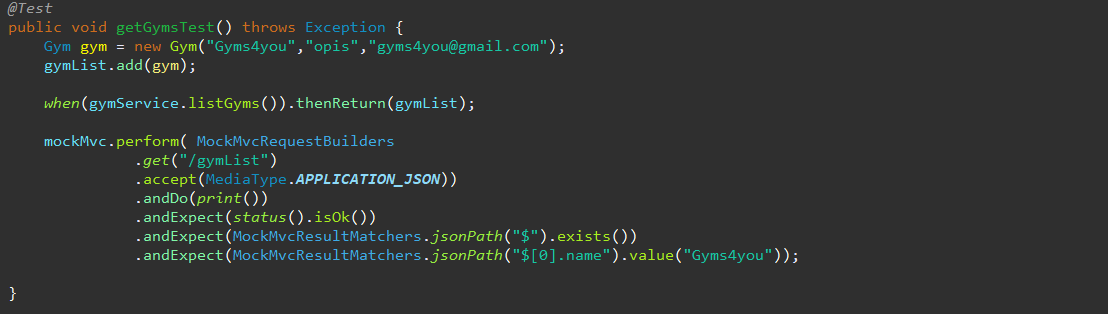
\includegraphics[scale=0.5]{slike/getGyms.PNG} %veličina slike u odnosu na originalnu datoteku i pozicija slike
    			\centering
    			\label{fig:promjene}
    	    \end{figure}
	

			\noindent \underbar{\textbf{2. Dodaj novu teretanu}}
			
            Ovdje smo testirali pokušaj dodavanja nove teretane odlaskom na /addGym  dok smo ulogirani kao role owner.

			\begin{figure}[H]
    			\hspace*{-1.5cm}
    			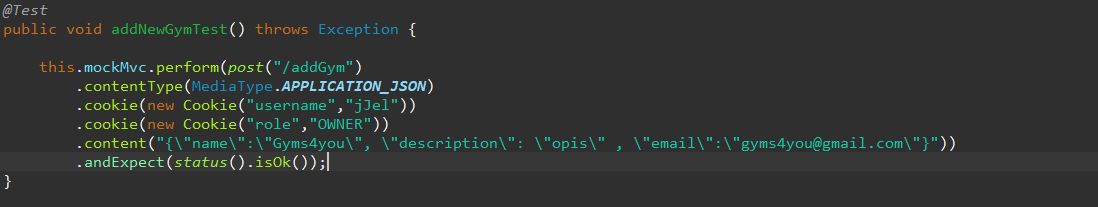
\includegraphics[scale=0.5]{slike/addNewGym.PNG} %veličina slike u odnosu na originalnu datoteku i pozicija slike
    			\centering
    			\label{fig:promjene}
    	    \end{figure}
	

			\noindent \underbar{\textbf{3. Dohvati trenerovu teretanu}}
			
			Ovdje smo testirali pokušaj dohvaćanja teretane u kojoj radi određeni trener odlaskom na /myGyms sa trenutnim ulogiranim trenerom.

			\begin{figure}[H]
    			\hspace*{-1.5cm}
    			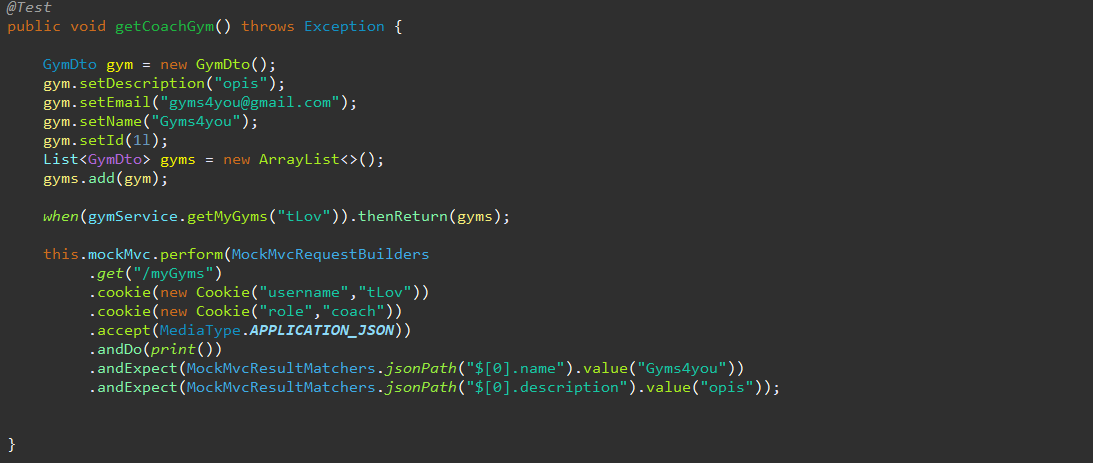
\includegraphics[scale=0.5]{slike/getCoachGym.PNG} %veličina slike u odnosu na originalnu datoteku i pozicija slike
    			\centering
    			\label{fig:promjene}
    	    \end{figure}
	
				
			\noindent \underbar{\textbf{4. Dohvati informacije o teretani}}
			
			Ovdje smo testirali pokušaj dohvaćanja informacija o određeneoj teretani odlaskom na /gymInfo sa pripadnim parametrom id koji se šalje preko URL-a.
             
			\begin{figure}[H]
    			\hspace*{-1.5cm}
    			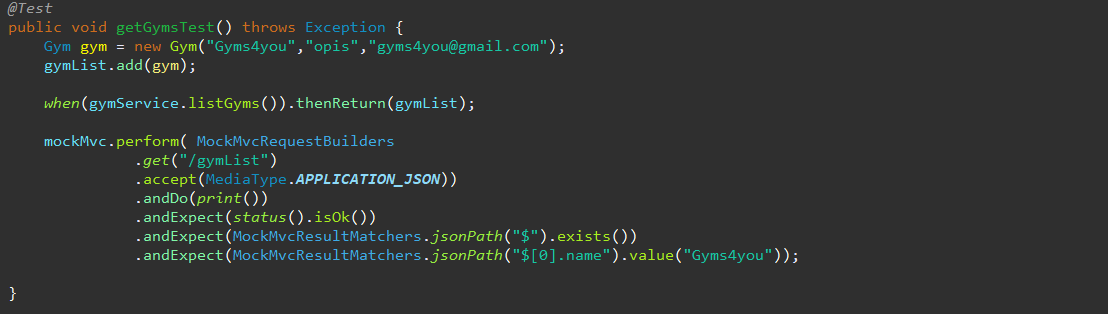
\includegraphics[scale=0.5]{slike/getGyms.PNG} %veličina slike u odnosu na originalnu datoteku i pozicija slike
    			\centering
    			\label{fig:promjene}
    	    \end{figure}
	

			\noindent \underbar{\textbf{5. Pronađi trenera}}
			
			Ovdje smo testirali pokušaj dohvaćanja trenera odlaskom na /coach sa pripadnim parametrom username koji se šalje preko URL-a.

			\begin{figure}[H]
    			\hspace*{-1.5cm}
    			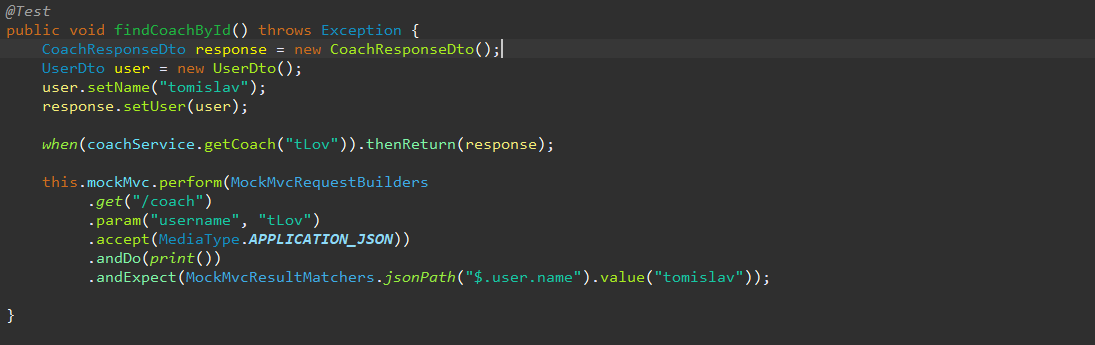
\includegraphics[scale=0.5]{slike/findCoachBy.PNG} %veličina slike u odnosu na originalnu datoteku i pozicija slike
    			\centering
    			\label{fig:promjene}
    	    \end{figure}
	

				
			\noindent \underbar{\textbf{6. Pronađi trenera (error) }}
			
			 Ovdje smo testirali pokušaj dohvaćanja trenera odlaskom na /coach bez parametra username kako bi dobili response 4xx koji javlja da je došlo do pogreške.
			\begin{figure}[H]
    			\hspace*{-1.5cm}
    			
\includegraphics[scale=0.5]{slike/findCoachByError.PNG} %veličina slike u odnosu na originalnu datoteku i pozicija slike
    			\centering
    			\label{fig:promjene}
    	    \end{figure}
	

				
			\noindent \underbar{\textbf{Prikaz prolaza svih ispita}}

			\begin{figure}[H]
    			\hspace*{-1.5cm}
    			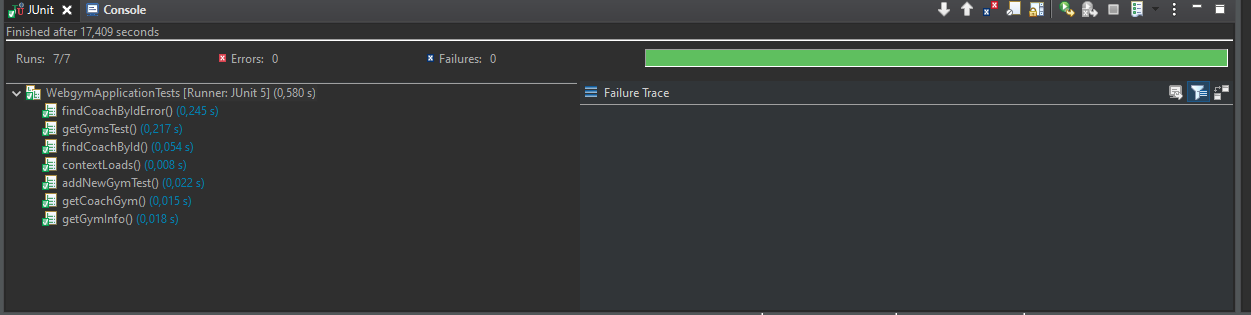
\includegraphics[scale=0.5]{slike/rezultati.PNG} %veličina slike u odnosu na originalnu datoteku i pozicija slike
    			\centering
    			\label{fig:promjene}
    	    \end{figure}
	

			\subsection{Ispitivanje sustava}
			
			 \textit{Potrebno je provesti i opisati ispitivanje sustava koristeći radni okvir . Razraditi \textbf{minimalno 4 ispitna slučaja} u kojima će se ispitati redovni slučajevi, rubni uvjeti te poziv funkcionalnosti koja nije implementirana/izaziva pogrešku kako bi se vidjelo na koji način sustav reagira kada nešto nije u potpunosti ostvareno. Ispitni slučaj se treba sastojati od ulaza (npr. korisničko ime i lozinka), očekivanog izlaza ili rezultata, koraka ispitivanja i dobivenog izlaza ili rezultata.\\ }
			 
		
		 	 Za ispitivanje funkcionalnosti sustava koristili smo Selenium IDE. Testirali smo
		 	 sve obrazce uporabe te smo prolazili kroz aplikaciju i gledali općenito ponašanje
		 	 u nadi da pronađemo neko neočekivano hazardno ponašanje u svrhu otklonuća problema.
		 	 Neke od testiranih obrazaca uporabe smo prikazali u nastavku. ( UC1, UC2, UC3, UC7).
		 	 
		 	 
	
	            \noindent \underbar{\textbf{1. Ispitni slučaj (UC1 : Pregled teretana)}}
                \begin{packed_item}
						\item  \textbf{Ulaz : } 
						\item[] \begin{packed_enum}
	
							\item korisnik je pritisnuo na "popis teretana"

						\end{packed_enum}
						\item  \textbf{Očekivani rezultat: } 
						\item[] \begin{packed_enum}
	
							\item korisnik je dobio prikaz svih teretana

						\end{packed_enum}
						
						\item  \textbf{rezultat : }
						\item[] \begin{packed_enum}
	
							\item rezultat je jednak očekivanom rezultatu.

						\end{packed_enum}

				\end{packed_item}
				
				\begin{figure}[H]
        			\hspace*{-1.5cm}
        			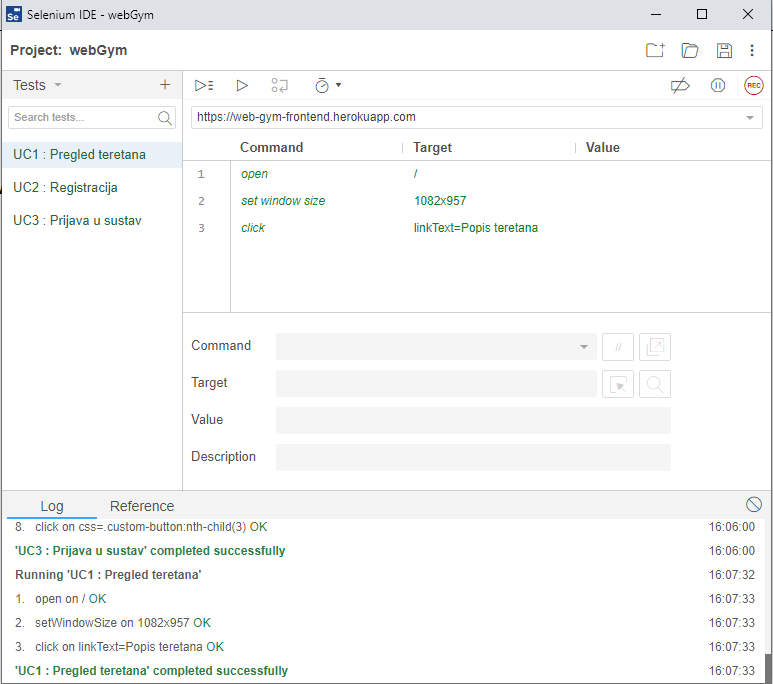
\includegraphics[scale=0.5]{dijagrami/UC1.PNG} %veličina slike u odnosu na originalnu datoteku i pozicija slike
        			\centering
        			\label{fig:promjene}
	        	\end{figure}
				
				\noindent \underbar{\textbf{2. Ispitni slučaj (UC2 : Registracija korisnika)}}
                \begin{packed_item}
						\item  \textbf{Ulaz : } 
						\item[] \begin{packed_enum}
	
							\item korisnik je pritisnuo na "prijava"
							\item korisnik je ispunio obrazac "registracija"
							\item korisnik je pritisnuo "registriraj"

						\end{packed_enum}
						\item  \textbf{Očekivani rezultat: } 
						\item[] \begin{packed_enum}
	
							\item korisnik se uspješno registrirao i spremio u bazu podataka

						\end{packed_enum}
						
						\item  \textbf{rezultat : }
						\item[] \begin{packed_enum}
	
							\item rezultat je jednak očekivanom rezultatu.

						\end{packed_enum}

				\end{packed_item}
				
				\begin{figure}[H]
        			\hspace*{-1.5cm}
        			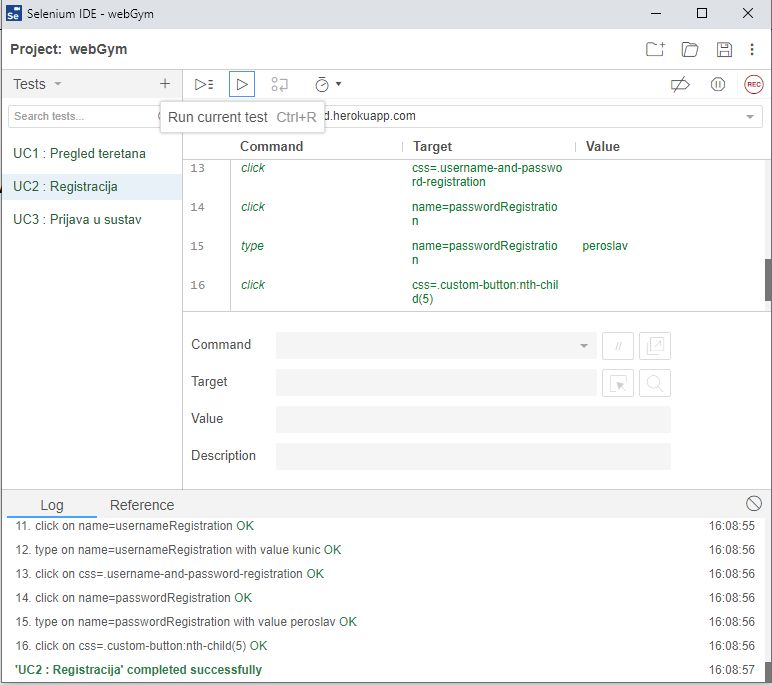
\includegraphics[scale=0.5]{dijagrami/UC2.PNG} %veličina slike u odnosu na originalnu datoteku i pozicija slike
        			\centering
        			\label{fig:promjene}
	        	\end{figure}
				
				\noindent \underbar{\textbf{3. Ispitni slučaj (UC3 : Prijava u sustav)}}
                \begin{packed_item}
						\item  \textbf{Ulaz : } 
						\item[] \begin{packed_enum}
	
							\item korisnik je pritisnuo na "prijava"
							\item korisnik je ispunio obrazac "prijava"
							\item korisnik je pritisnuo "prijava"

						\end{packed_enum}
						\item  \textbf{Očekivani rezultat: } 
						\item[] \begin{packed_enum}
	
							\item korisnik se uspješno prijavio u sustav

						\end{packed_enum}
						
						\item  \textbf{rezultat : }
						\item[] \begin{packed_enum}
	
							\item rezultat je jednak očekivanom rezultatu.

						\end{packed_enum}

				\end{packed_item}
				
				\begin{figure}[H]
        			\hspace*{-1.5cm}
        			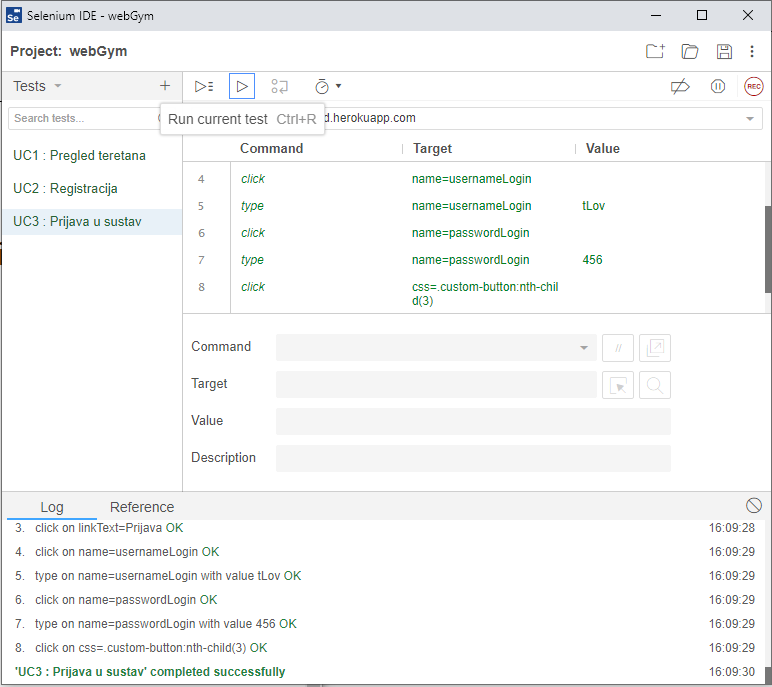
\includegraphics[scale=0.5]{dijagrami/UC3.PNG} %veličina slike u odnosu na originalnu datoteku i pozicija slike
        			\centering
        			\label{fig:promjene}
	        	\end{figure}
				
				\noindent \underbar{\textbf{4. Ispitni slučaj (UC7 : Pregled specifične teretane)}}
                \begin{packed_item}
						\item  \textbf{Ulaz : } 
						\item[] \begin{packed_enum}
	
							\item korisnik je pritisnuo na "Popis teretana"
							
							\item korisnik je pritisnuo na gumb informacije

						\end{packed_enum}
						\item  \textbf{Očekivani rezultat: } 
						\item[] \begin{packed_enum}
	
							\item korisnik je dobio informacije o odabranoj teretani

						\end{packed_enum}
						
						\item  \textbf{rezultat : }
						\item[] \begin{packed_enum}
	
							\item rezultat je jednak očekivanom rezultatu.

						\end{packed_enum}

				\end{packed_item}
					\begin{figure}[H]
        			\hspace*{-1.5cm}
        			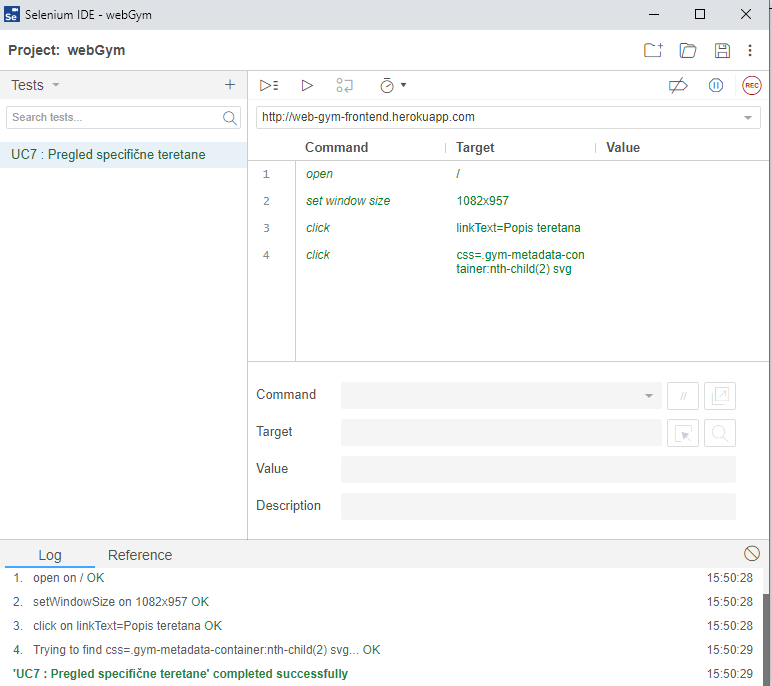
\includegraphics[scale=0.5]{slike/teretana.PNG} %veličina slike u odnosu na originalnu datoteku i pozicija slike
        			\centering
        			\label{fig:promjene}
	        	\end{figure}
	        	
	        \noindent \underbar{\textbf{5. Ispitni slučaj (UC20 : Pregled trenereove ponude)}}
                \begin{packed_item}
						\item  \textbf{Ulaz : } 
						\item[] \begin{packed_enum}
	
							\item trener je pritisnuo na "Moji planovi"

						\end{packed_enum}
						\item  \textbf{Očekivani rezultat: } 
						\item[] \begin{packed_enum}
	
							\item trener je dobio prikaz svih svojih planova treninga

						\end{packed_enum}
						
						\item  \textbf{rezultat : }
						\item[] \begin{packed_enum}
	
							\item došlo je do pogreške te se nisu učitali trenerovi planovi.
                                                
                            - Test je napravljen prije implementiranja mogućnosti trenera da pregleda svoje planove treninga i prehrane , do greške je došlo zbog problema u pamćenju cookie-a koje smo naknadno riješili.
                        
						\end{packed_enum}

				\end{packed_item}
					\begin{figure}[H]
        			\hspace*{-1.5cm}
        			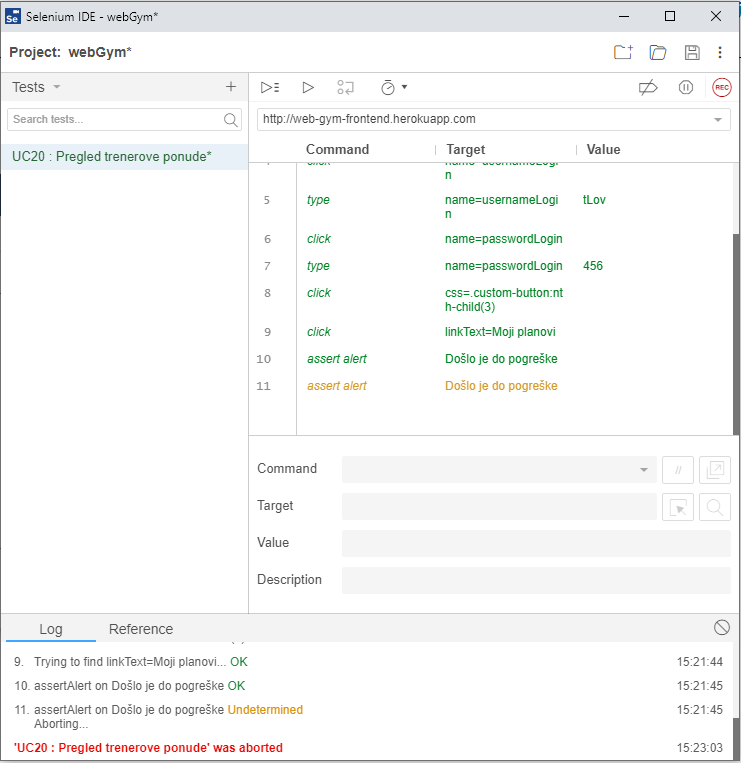
\includegraphics[scale=0.5]{slike/error.PNG} %veličina slike u odnosu na originalnu datoteku i pozicija slike
        			\centering
        			\label{fig:promjene}
	        	\end{figure}
		 
			\eject 
			
			
		\section{Dijagram razmještaja}
		
		 \textit{Potrebno je umetnuti \textbf{specifikacijski} dijagram razmještaja i opisati ga. Moguće je umjesto specifikacijskog dijagrama razmještaja umetnuti dijagram razmještaja instanci, pod uvjetom da taj dijagram bolje opisuje neki važniji dio sustava.}
		
		Dijagram razmještaja prikazuje generalnu topologiju sustava koji se koristi kako bi resursi bili optimalno raspoređeni. Predstavlja statički pogled na razmještaj sklopovskih i programskih komponenata. Na poslužiteljskom računalu se nalaze web poslužitelj, poslužitelj baze podataka i poslužitelj za frontend. Klijenti koriste web preglednik kako bi pristupili web aplikaciji. U bazi podataka sadržane su sve potrebne informacije i datoteke koje korisnik može zahtijevati. Sustav je baziran na arhitekturi ”klijent – poslužitelj”. Komunikacija između poslužiteljskog računala i klijentskog računala se omogućuje HTTP protokolom. 
		
		
		
		\begin{figure}[h]
			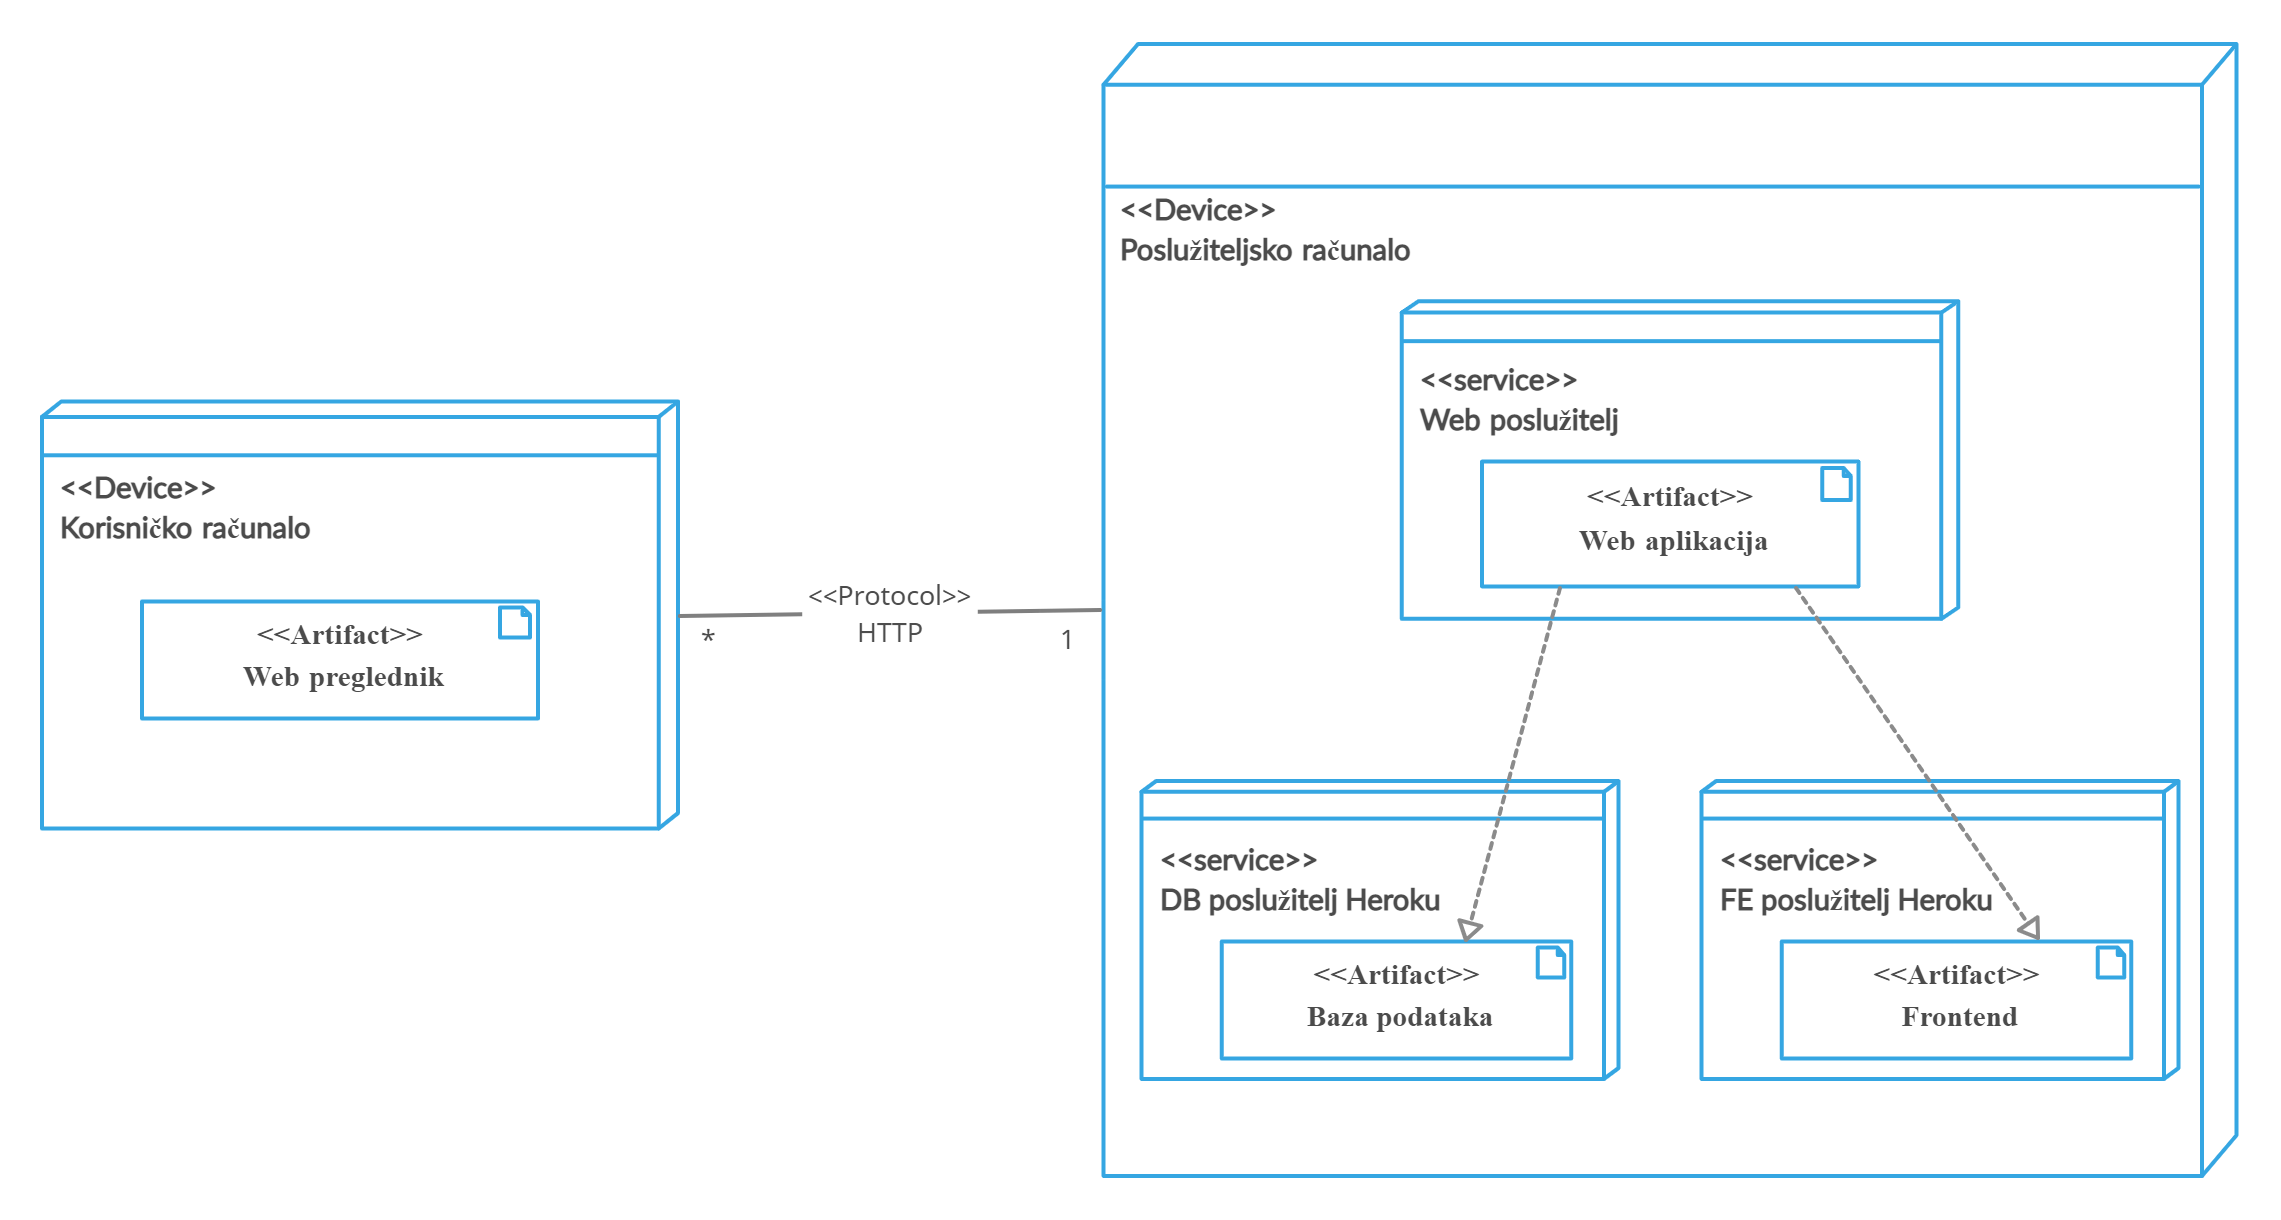
\includegraphics[height=                       9cm,width=1\textwidth]{dijagrami/Dijagram_razmjestaja.png}
			\begin{center}
				Slika 5.1: Dijagram razmještaja
			\end{center}
		\end{figure}
		
		\eject	
		
		
		\section{Upute za puštanje u pogon}

		    \begin{packed_item}
						\item  \textbf{1. Stvaranje backend heroku servera} 
						\item[] \begin{packed_enum}
	
							\item Stvaranje account-a na https://dashboard.heroku.com/
							
							\item Instalacija Heroku CLI : https://devcenter.heroku.com/articles/heroku-cli
							
							\item Otvaranje command prompt-a
							
							\item Upiši "heroku create "NAME-OF-APP" (webGym) ili samo "heroku create"
							
							    - U slučaju da se ne navede ime aplikacije , i dalje će se stvoriti server ali s random imenom koji je kasnije moguće preimenovati u željeno ime.
							
							\item Stvoren je server.
							    
							    \begin{figure}[H]
                        			\hspace*{-1.5cm}
                        			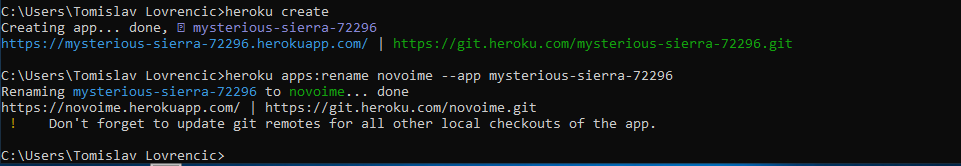
\includegraphics[scale=0.5]{dijagrami/cmd.PNG} %veličina slike u odnosu na originalnu datoteku i pozicija slike
                        			\centering
                        			\label{fig:promjene}
                        		\end{figure}

						\end{packed_enum}
						\item  \textbf{2. Konfiguracija baze podataka} 
						\item[] \begin{packed_enum}
	
							\item Odlazak na stranicu  https://dashboard.heroku.com/
							
							\item Klik na stvoreni server. (novoime)
							
							\item Klik na resources
							
							\item Pronaći pod add-ons  Heroku POSTGRES
							
							    - Odabrati Hobby dev - FREE
							  
							
							\item Stisnuti na SUBMIT FORM.
							
							\item Stvorena je baza podataka
							    
							    \begin{figure}[H]
                        			\hspace*{-1.5cm}
                        			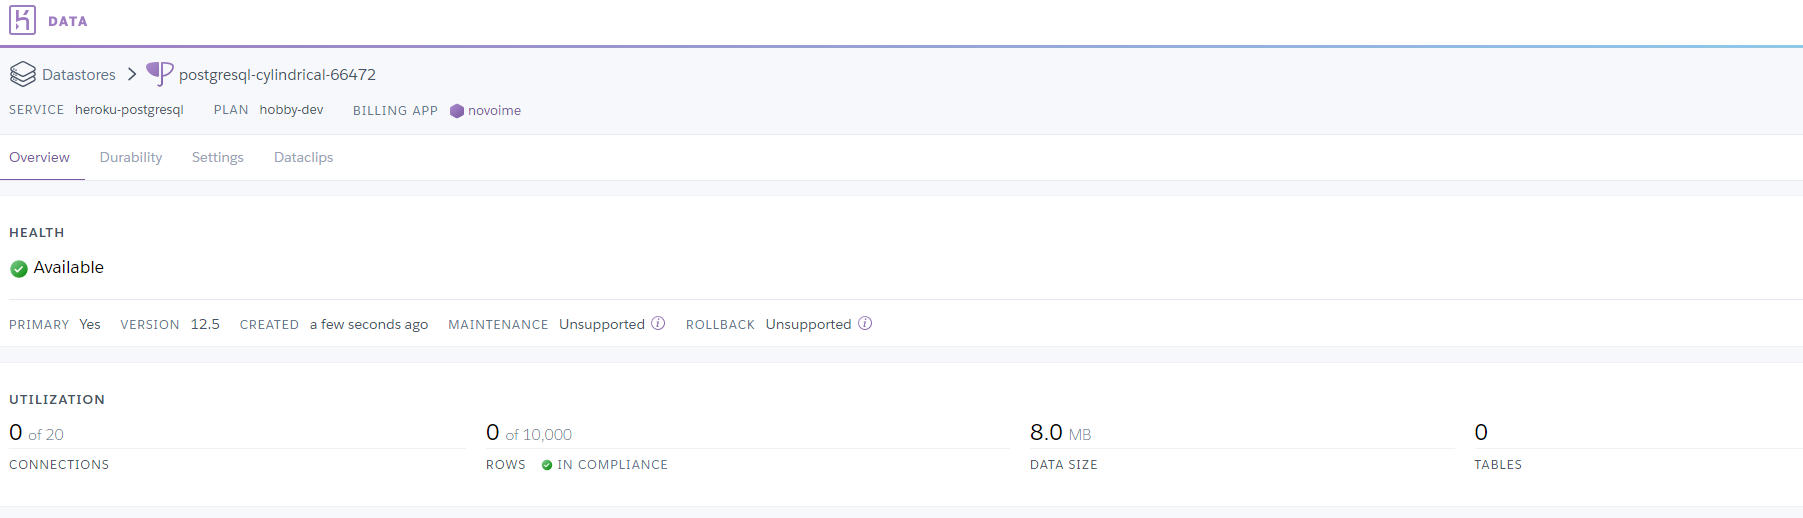
\includegraphics[scale=0.3]{dijagrami/baza.PNG} %veličina slike u odnosu na originalnu datoteku i pozicija slike
                        			\centering
                        			\label{fig:promjene}
                        		\end{figure}

						\end{packed_enum}
						
						
						\item  \textbf{3. Spajanje backend server na stvorenu bazu u heroku}
						\item[] \begin{packed_enum}
	
							\item Odlazak na stranicu  https://dashboard.heroku.com/
							
							\item Klik na stvoreni server. (novoime)
							
							\item Klik na resources
							
							\item Klik na Heroku POSTGRES
							
							\item Klik na settings
							
							\item Klik na view credentials
							
							\item Otvori backend kod (java)
							
							\item Odi u src/main/resources/application.properties
							
							\item Podesi :
							    
							       - Potrebno je podesiti backend tako da se povezuje sa bazom koju smo u prethodnom koraku stvorili na heroku.
							       
							       - U tom naumu ćemo morati podesiti spring.datasource.url , spring.datasource.username te spring.datasource.password na način da ćemo pročitati vrijednosti koje nam je dao heroku credentials i nadodati ih na spomenute vrijednosti.
							       
							       - Zadnja napomena je dodavanje "jdbc:" na početak URI-a koje nam je generirao heroku.
						
							    \begin{figure}[H]
                        			\hspace*{-1.5cm}
                        			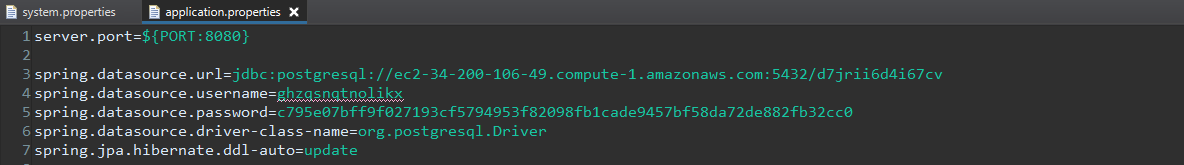
\includegraphics[scale=0.5]{slike/java.PNG} %veličina slike u odnosu na originalnu datoteku i pozicija slike
                        			\centering
                        			\label{fig:promjene}
                        		\end{figure}

						\end{packed_enum}
						
						\item  \textbf{4. deploy backend-a}
						\item[] \begin{packed_enum}
	
							\item Otvoriti backend project.
							
							\item Otvoriti pom.xml te dodati ovaj plugin.
			
							    \begin{figure}[H]
                        			\hspace*{-1.5cm}
                        			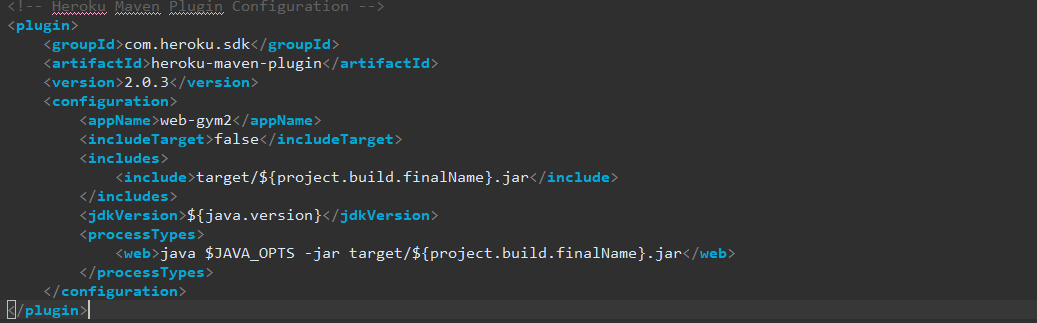
\includegraphics[scale=0.5]{slike/plugin.PNG} %veličina slike u odnosu na originalnu datoteku i pozicija slike
                        			\centering
                        			\label{fig:promjene}
                        		\end{figure}
                        		
                        		- Napomena : u našem slučaju prateći sve ove korake bi treabli napisati
                        		pod appName "novoime", dok nam je za projekt ime aplikacije ,kao što možemo vidjeti na slici "web-gym2".
							
							\item Otvoriti cmd te se pozicionirati u root backend projekta
							
							\item Napisati "mvn clean heroku:deploy"
						

						\end{packed_enum}
						
				\item  \textbf{5. Stvaranje frontend servera te deploy frontend-a}
				\item[] \begin{packed_enum}
	
							\item Odlazak na stranicu  https://dashboard.heroku.com/
							
							\item Otvoriti cmd te upisati "heroku create NAME-OF-FRONTEND-APP --buildpack https://github.com/mars/create-react-app-buildpack.git"

							\item Napraviti prazan folder , unutar foldera u cmd-u napisati "git init"
							
							\item U cmd-u napisati "heroku git:remote -a NAME-OF-FRONTEND-APP"
							
							\item Prekopirati root frontend projekta u stvoreni folder
							
							\item Dodati static.json datoteku u root frontend projekta
							    
							    \begin{figure}[H]
                        			\hspace*{-1.5cm}
                        			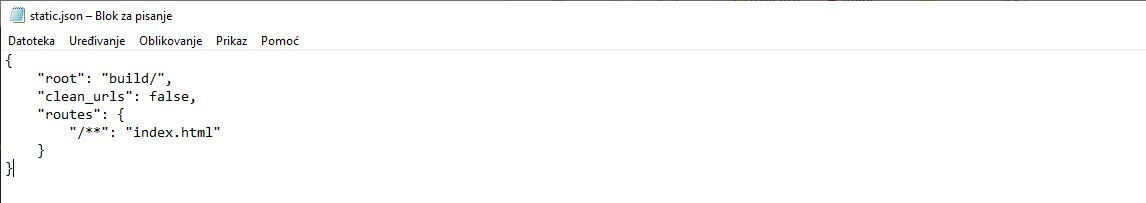
\includegraphics[scale=0.5]{slike/json.PNG} %veličina slike u odnosu na originalnu datoteku i pozicija slike
                        			\centering
                        			\label{fig:promjene}
                        		\end{figure}
							
							\item prije deploya frontenda , ući u src/App.js te promjeniti backendURL i 
							postaviti ga na server backenda.
							
							    \begin{figure}[H]
                        			\hspace*{-1.5cm}
                        			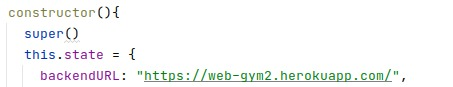
\includegraphics[scale=0.7]{slike/front.png} %veličina slike u odnosu na originalnu datoteku i pozicija slike
                        			\centering
                        			\label{fig:promjene}
                        		\end{figure}
							
							\item U cmd- napisati "git add ."
							
							\item U cmd- napisati "git add -m "initial commit""
							
							\item U cmd- napisati "git push heroku master"
	

						\end{packed_enum}

				\end{packed_item}
				
			\eject 